\documentclass[twoside,nohyper]{tufte-book}

% ams
\usepackage{amssymb,amsmath}

\usepackage{ifxetex,ifluatex}
\usepackage{fixltx2e} % provides \textsubscript
\ifnum 0\ifxetex 1\fi\ifluatex 1\fi=0 % if pdftex
  \usepackage[T1]{fontenc}
  \usepackage[utf8]{inputenc}
\else % if luatex or xelatex
  \makeatletter
  \@ifpackageloaded{fontspec}{}{\usepackage{fontspec}}
  \makeatother
  \defaultfontfeatures{Ligatures=TeX,Scale=MatchLowercase}
  \makeatletter
  \@ifpackageloaded{soul}{
     \renewcommand\allcapsspacing[1]{{\addfontfeature{LetterSpace=15}#1}}
     \renewcommand\smallcapsspacing[1]{{\addfontfeature{LetterSpace=10}#1}}
   }{}
  \makeatother

\fi

% graphix
\usepackage{graphicx}
\setkeys{Gin}{width=\linewidth,totalheight=\textheight,keepaspectratio}

% booktabs
\usepackage{booktabs}

% url
\usepackage{url}

% hyperref
\usepackage{hyperref}

% units.
\usepackage{units}


\setcounter{secnumdepth}{2}

% citations
\usepackage{natbib}
\bibliographystyle{abbrvnat}


% pandoc syntax highlighting

% table with pandoc
\usepackage{longtable,booktabs,array}
\usepackage{calc} % for calculating minipage widths
% Correct order of tables after \paragraph or \subparagraph
\usepackage{etoolbox}
\makeatletter
\patchcmd\longtable{\par}{\if@noskipsec\mbox{}\fi\par}{}{}
\makeatother
% Allow footnotes in longtable head/foot
\IfFileExists{footnotehyper.sty}{\usepackage{footnotehyper}}{\usepackage{footnote}}
\makesavenoteenv{longtable}

% multiplecol
\usepackage{multicol}

% strikeout
\usepackage[normalem]{ulem}

% morefloats
\usepackage{morefloats}


% tightlist macro required by pandoc >= 1.14
\providecommand{\tightlist}{%
  \setlength{\itemsep}{0pt}\setlength{\parskip}{0pt}}

% title / author / date
\title{Data Analytics in Football: Pitch Control and Beyond}
\author{Álvaro Novillo Correas}
\date{2024-02-04}

\geometry{
  a4paper,
  top=2.5cm,
  bottom=2.5cm,
  inner=3cm,
  outer=3cm
}
\usepackage{pdfpages}


\renewcommand{\baselinestretch}{1.15}
\parskip=6pt

\definecolor{azulUC3M}{RGB}{0,0,102}
\definecolor{gray97}{gray}{.97}
\definecolor{gray75}{gray}{.75}
\definecolor{gray45}{gray}{.45}

\usepackage[a-1b]{pdfx}

\usepackage{hyperref}
\hypersetup{colorlinks=true,
	linkcolor=black, % enlaces a partes del documento (p.e. índice) en color negro
	urlcolor=blue} % enlaces a recursos fuera del documento en azul


\usepackage{amsmath,amssymb,amsfonts,amsthm}

\usepackage{txfonts} 
\usepackage[T1]{fontenc}
\usepackage[utf8]{inputenc}

\usepackage[english]{babel} 
\usepackage[babel, english=american]{csquotes}
\AtBeginEnvironment{quote}{\small}

% diseño de PIE DE PÁGINA
\usepackage{fancyhdr}
\pagestyle{fancy}
\fancyhf{}
\renewcommand{\headrulewidth}{0pt}
\rfoot{\thepage}
\fancypagestyle{plain}{\pagestyle{fancy}}


\usepackage{titlesec}
\usepackage{titletoc}
\titleformat{\chapter}[block]
{\large\bfseries\filcenter}
{\thechapter.}
{5pt}
{\MakeUppercase}
{}
\titlespacing{\chapter}{0pt}{0pt}{*3}
\titlecontents{chapter}
[0pt]                                               
{}
{\contentsmargin{0pt}\thecontentslabel.\enspace\uppercase}
{\contentsmargin{0pt}\uppercase}                        
{\titlerule*[.7pc]{.}\contentspage}                 

\titleformat{\section}
{\bfseries}
{\thesection.}
{5pt}
{}
\titlecontents{section}
[5pt]                                               
{}
{\contentsmargin{0pt}\thecontentslabel.\enspace}
{\contentsmargin{0pt}}
{\titlerule*[.7pc]{.}\contentspage}

\titleformat{\subsection}
{\normalsize\bfseries}
{\thesubsection.}
{5pt}
{}
\titlecontents{subsection}
[10pt]                                               
{}
{\contentsmargin{0pt}                          
	\thecontentslabel.\enspace}
{\contentsmargin{0pt}}                        
{\titlerule*[.7pc]{.}\contentspage}  



\usepackage{multirow} %permite combinar celdas 
\usepackage{caption} %para personalizar el título de tablas y figuras
\usepackage{floatrow} %utilizamos este paquete y sus macros \ttabbox y \ffigbox para alinear los nombres de tablas y figuras de acuerdo con el estilo definido. Para su uso ver archivo de ejemplo 
\usepackage{array} % con este paquete podemos definir en la siguiente línea un nuevo tipo de columna para tablas: ancho personalizado y contenido centrado
\newcolumntype{P}[1]{>{\centering\arraybackslash}p{#1}}
\DeclareCaptionFormat{upper}{#1#2\uppercase{#3}\par}


% Diseño de tabla para ingeniería
\captionsetup[table]{
	format=upper,
	justification=centering,
	labelsep=period,
	width=.75\linewidth,
	labelfont=small,
	font=small,
}




\usepackage{graphicx}
\graphicspath{{imagenes/}} %ruta a la carpeta de imágenes

% Diseño de figuras para ingeniería
\captionsetup[figure]{
	format=hang,
	name=Fig.,
	singlelinecheck=off,
	labelsep=period,
	labelfont=small,
	font=small		
}




\usepackage{chngcntr}
\counterwithout{footnote}{chapter}


\usepackage{listings}


\lstdefinestyle{estilo}{ frame=Ltb,
	framerule=0pt,
	aboveskip=0.5cm,
	framextopmargin=3pt,
	framexbottommargin=3pt,
	framexleftmargin=0.4cm,
	framesep=0pt,
	rulesep=.4pt,
	backgroundcolor=\color{gray97},
	rulesepcolor=\color{black},
	%
	basicstyle=\ttfamily\footnotesize,
	keywordstyle=\bfseries,
	stringstyle=\ttfamily,
	showstringspaces = false,
	commentstyle=\color{gray45},     
	%
	numbers=left,
	numbersep=15pt,
	numberstyle=\tiny,
	numberfirstline = false,
	breaklines=true,
	xleftmargin=\parindent
}

\captionsetup[lstlisting]{font=small, labelsep=period}

\lstset{style=estilo}
\renewcommand{\lstlistingname}{\uppercase{Código}}

% Define the color azulUC3M
\definecolor{azulUC3M}{RGB}{0,0,102}

% Redefine \maketitle
\makeatletter
\renewcommand{\maketitle}{%
	\begin{titlepage}
		\begin{sffamily}
			\color{azulUC3M}
			\begin{center}
				
\includegraphics[width=16cm]{imagenes/Portada_Logo.png}\\[1cm]
				\begin{Large}
					Master Degree in...\\			
					Academic Year (e.g., 2018-2019)\\
					\vspace{1cm}		
					\textsl{Master Thesis}\\
					\bigskip
				\end{Large}
				{\Huge Data Analytics in Football: Pitch Control and Beyond}\\
				\vspace*{0.5cm}
				\rule{10.5cm}{0.1mm}\\
				\vspace*{0.9cm}
				{\LARGE Author's complete name}\\ 
				\vspace*{1cm}
				\begin{Large}
					1st Tutor complete name\\
					2nd Tutor complete name\\
					Place and date\\
				\end{Large}
			\end{center}

			\vfill
			\color{black}
			\begin{footnotesize}
				\noindent\fbox{
					\begin{minipage}{\textwidth}
						\textbf{AVOID PLAGIARISM}\\
						The University uses the \textbf{Turnitin Feedback Studio} program within the Aula Global for the delivery of student work. This program compares the originality of the work delivered by each student with millions of electronic resources and detects those parts of the text that are copied and pasted. Plagiarizing in a TFM is considered a \textbf{Serious Misconduct}, and may result in permanent expulsion from the University.
					\end{minipage}	
				}
				\vspace*{.5cm}\\	
				\noindent
\includegraphics[width=4.2cm]{imagenes/creativecommons.png}\\
				\emph{[Include this code in case you want your Master Thesis published in Open Access University Repository]}\\
				This work is licensed under Creative Commons \textbf{Attribution – Non Commercial – Non Derivatives}
			\end{footnotesize}
		\end{sffamily}
	\end{titlepage}
}
\makeatother



\begin{document}

\maketitle



{
\setcounter{tocdepth}{1}
\tableofcontents
}

\hypertarget{dedication}{%
\chapter*{Dedication}\label{dedication}}
\addcontentsline{toc}{chapter}{Dedication}

\listoffigures

\hypertarget{introduction.-data-analytics-in-football}{%
\chapter{Introduction. Data Analytics in football}\label{introduction.-data-analytics-in-football}}

The digital revolution is currently one of the most significant
challenges of our time, altering numerous aspects of society. Football,
in particular, has also been influenced by this transformation.
Technological advancements and digitalization have resulted in a swift
upsurge in the number of measuring devices, data collection and volumes
of data. The leading data companies worldwide, including IBM, Intel, SAP
and Microsoft, are vying for superior data analytics tools and
leveraging sports as an example domain to showcase their products and
brand power \citep{1}.

The practice of data analytics in football has a long history, dating
back to the post-World War II era, when data collection and analysis was
undertaken manually using pencil and paper \citep{1}. It wasn't until
Moneyball was published in 2003 that significant progress began to
emerge: The book, "The Art of Winning an Unfair Game" introduced
sports analytics to a broader audience. It illustrated the use of data
analytics in identifying undervalued players and constructing a
successful team. Since then, data analytics has become an integral
component of sport, football inclusive \citep{1}.

One of the best examples of data analytics being applied to sports is
basketball. Teams use data to analyze player performance, identify
strengths and weaknesses, and develop strategies to win games \citep{2}. They
use in-memory analytics, visualization, the cloud, mobility, camera
footage, and sensors to transform their game. This performance analyses
are of vital importance to a team, aiming to reduce expenditure, enhance
team worth and refine processes across all levels and segments of
operations. The German Football Association (DFB) and the National
Basketball Association (NBA) are two unique cases of digital
transformation from the sports world. Successful teams turn player
performance data into action and gain a competitive advantage.

Over the last years, football analytics has gained significant
popularity, aiming to delve deeper into the game by utilizing advanced
data analysis techniques to optimize team and player performance. This
chapter examines the various areas of football where data can be used
for analysis, alongside the commonly found data types within this
industry.

\hypertarget{statistical-analysis-in-football}{%
\chapter{Statistical analysis in football}\label{statistical-analysis-in-football}}

When discussing sports analytics in football, the first metric that
often springs to mind is the Expected Goals (xG) ratio. This statistical
indicator is a predictive Machine Learning (ML) model used to assess the
likelihood of scoring for every shot made in the game. In the context of
each shot, the xG model computes the scoring probability, leveraging a
set of event parameters.

Wyscout xG model, for example, encompass the shot's spatial coordinates,
the assisting player's position, the striking player's use of foot or
head, the type of assist involved, the occurrence of a dribble by either
a field player or the goalkeeper immediately preceding the shot, whether
the shot arises from a set piece, whether it transpires during a
counterattack or in a transitional phase of play, and the subjective
assessment of shot danger as determined by a designated tagger. The
amalgamation of these parameters serves as the foundation for training
the xG model using historical Wyscout data, culminating in the
prediction of the likelihood of a given shot resulting in a goal
\citep{wyscout}.

The probabilities range from 0 to 1. Thus, a shot with an xG value of
0.1 has a 10\% chance of being scored. Penalties have a fixed xG value of
0.76.

\begin{figure}

{\centering 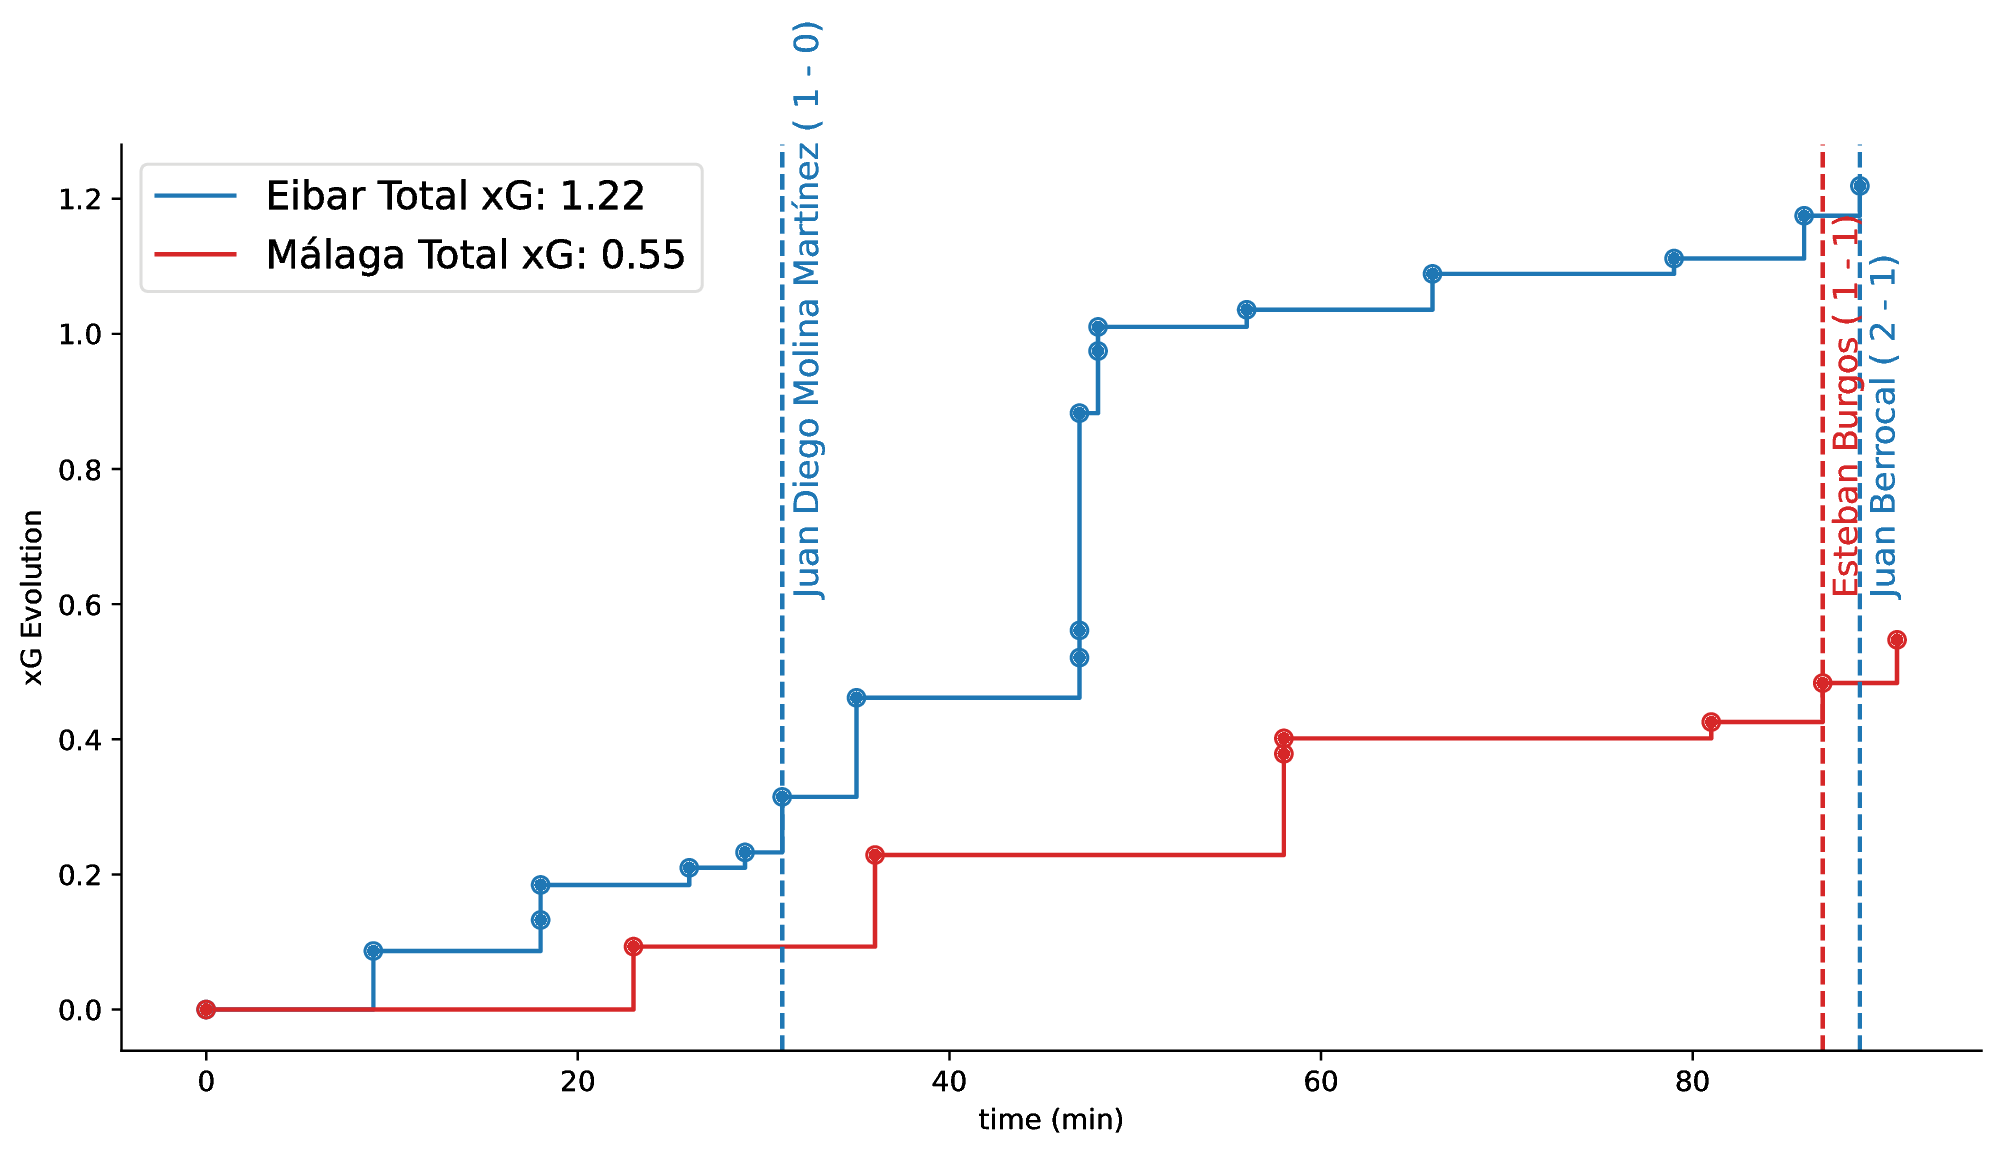
\includegraphics[width=0.8\linewidth]{imagenes/xg_evol} 

}

\caption{\label{fig:f2.1} Cumulative development of expected goals (xG) during the Eibar-Malaga match, held on January 15th in Spain’s second division. Each point denotes a shot made by both teams throughout the game. Vertical dashed lines indicate the goal scored, displaying the player and the corresponding score at that specific moment of the match.}\label{fig:unnamed-chunk-2}
\end{figure}

Fig. provides a
visual representation of the cumulative development of expected goals
(xG) during the Eibar - Malaga match, which took place on January 15th,
2023 in Spain's second division. Each data point on the graph
corresponds to a shot made by both teams over the course of the game,
offering a comprehensive overview of the evolving scoring opportunities
and outcomes throughout the duration of the game.

\bibliography{bibliografia.bib}



\end{document}
